\documentclass[nofootinbib,aip,jcp,reprint]{revtex4-1}

\usepackage{graphicx}
%\usepackage{enumitem,booktabs,cfr-lm}
%\usepackage{enumitem,cfr-lm}

\usepackage{enumitem}
\usepackage[referable]{threeparttablex}
\renewlist{tablenotes}{enumerate}{1}
\makeatletter
\setlist[tablenotes]{label=\tnote{\alph*},ref=\alph*,itemsep=\z@,topsep=\z@skip,partopsep=\z@skip,parsep=\z@,itemindent=\z@,labelindent=\tabcolsep,labelsep=.2em,leftmargin=*,align=left,before={\footnotesize}}
\makeatother


\usepackage{mathtools}
\usepackage{graphicx}
\usepackage{color}
\usepackage{ulem}
\usepackage{caption}
\usepackage{subcaption}
\usepackage{array}

\interfootnotelinepenalty=10000
\usepackage{comment}
\usepackage[version-1-compatibility]{siunitx}
\usepackage{siunitx}
 \usepackage{url}

\usepackage{array}
\newcolumntype{C}[1]{>{\centering\arraybackslash}p{#1}}
\captionsetup[figure]{labelfont=bf,
                    textfont=normalfont,
                    justification=RaggedRight}
\captionsetup[table]{labelfont=bf,
                    textfont=normalfont,
                    justification=RaggedRight}
\usepackage{diagbox}

\usepackage{multirow}
\newcommand{\head}[1]{\textnormal{\textbf{#1}}}
\newcommand{\normal}[1]{\multicolumn{1}{l}{#1}}

\usepackage{booktabs}
\newcommand{\ra}[1]{\renewcommand{\arraystretch}{#1}}

\newcommand{\pp}{\textcolor{blue}}
\newcommand{\sk}{\textcolor{red}}

\begin{document}

\title{Optical-Pumping of AlH$^+$ molecules to a Single Hyperfine State in the Ground Rovibronic Manifold}

\author{Panpan Huang}
\affiliation{Department of Physics and Astronomy, Northwestern University, Evanston, IL 60208, USA}

\author{Schuyler Kain}
\affiliation{Department of Physics and Astronomy, Northwestern University, Evanston, IL 60208, USA}

\author{Antonio de Oliveira-Filho}
\affiliation{Departamento de Química, Faculdade de Filosofia, Ciências e Letras de Ribeirão Preto, Universidade de São Paulo, Ribeirão Preto-SP 14040-901, Brazil}

\author{Brian Odom}
\email{b-odom@northwestern.edu}
\affiliation{Department of Physics and Astronomy, Northwestern University, Evanston, IL 60208, USA}

\date{\today}

\begin{abstract}
In this work we propose an optical pumping scheme to cool Paul-trapped AlH$^+$ molecules to the stretched hyperfine state ($\lvert F=7/2, m_F=7/2\rangle$) of the rovibronic ground state ($\lvert X^2\Sigma^+, v=0, N=0\rangle$) using a combination of a linearly polarized and a circularly polarized broadband pulsed laser to cool down the rotational degree of freedom and drive the population to the stretched hyperfine state respectively. We assert that adding a laser to couple the $v=1 \rightarrow v=0$ transition in the  $ X^2\Sigma^+$ state can accelerate the cooling process. In support of our efforts, the hyperfine coupling constants of the $A^2\Pi$ state and the $X^2\Sigma^+$ state are calculated since the lasers couple the transitions between the hyperfine states of $\lvert X^2\Sigma^+, v=0\rangle$ and $\lvert A^{2}\Pi, v=0\rangle$ in AlH$^+$ but only some hyperfine constants of the $X^{2}\Sigma^+$ have been measured or calculated. Applying the calculated hyperfine structures in the simulation of population dynamics solving rate equations, we show that under optimum conditions, the population in the stretched hyperfine state of the rovibronic gorund state can reach $63.2\, \%$ after 80 {\micro}s (334.6 ms) and $95.4\, \%$ after 2.2 ms (1.280 s) with (without) the rovibrational coupling laser.
\end{abstract}

\maketitle
\begin{figure*}[!htp]
  \centering
  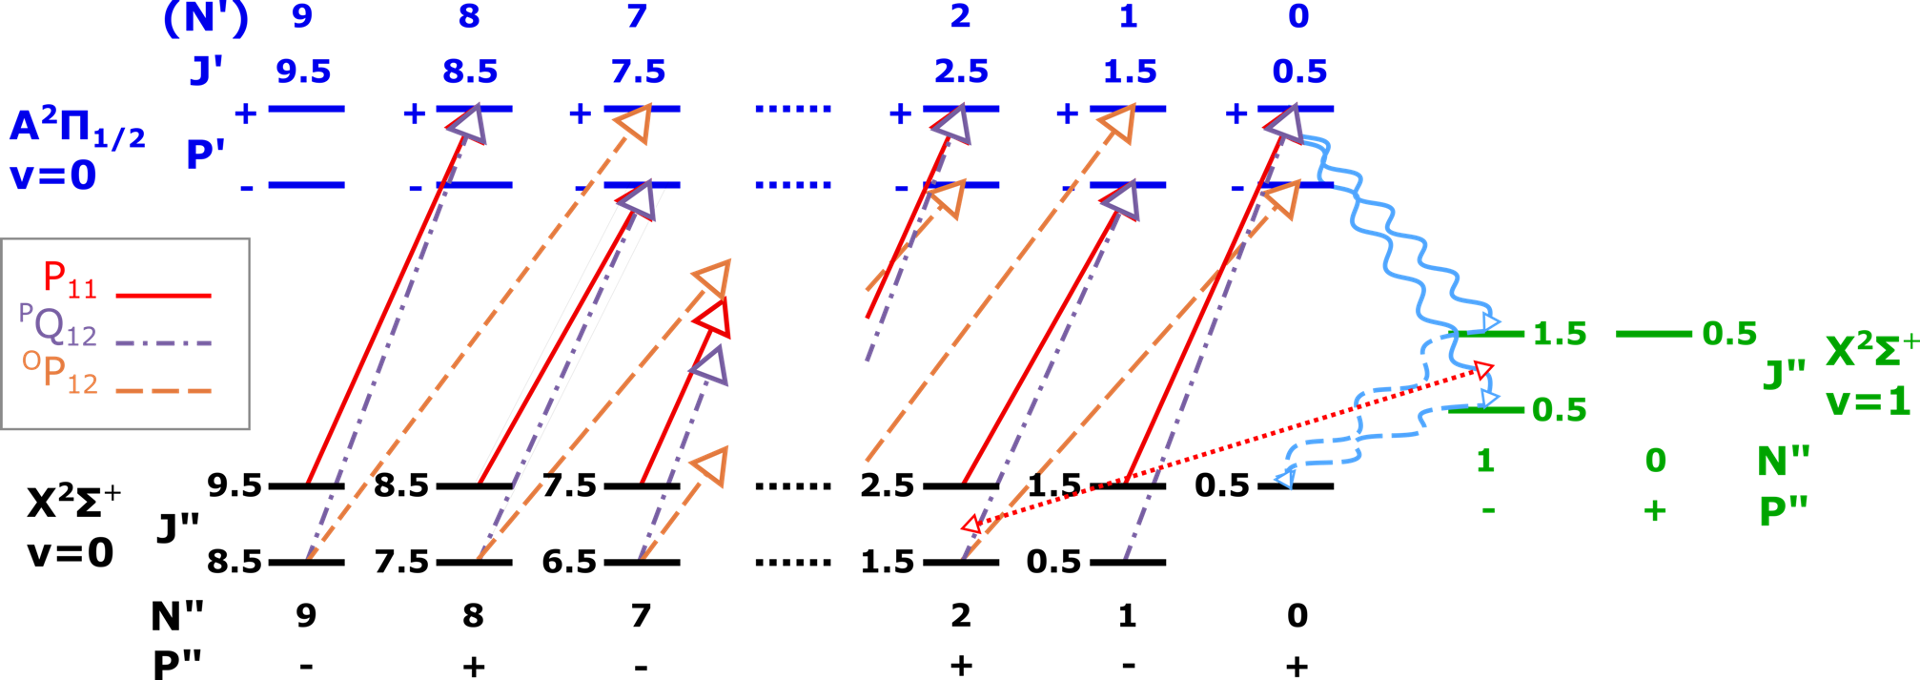
\includegraphics[width=14cm]{level_diagram_parity}
  \caption
  {Energy level structure of AlH$^+$ and the rotational cooling scheme. The rotational cooling laser drives $P_{11}$, $^PQ_{12}$ and $^OP_{11}$ branches from $\lvert X^2\Sigma^+, v=0\rangle$ to $\lvert A^2\Pi_{1/2}, v=0\rangle$. The time scale of the electronic relaxation without vibrational excitation from $\lvert A^2\Pi_{1/2}, v=0\rangle$ to $\lvert X^2\Sigma^+, v=0\rangle$ is around 60 $\mu$s. Solid curvy blue arrow indicates the electronic spontaneous relaxation with vibrational excitation. Dash curvy blue arrow indicates the rovibrational relaxation within the X state, which happens around the time scale of 140 ms. The rate of the population transferring from $v=1$ to $v=0$ in the X state is then limited by this time scale, which can be increased by adding the rovibrational coupling laser (indicated by the dashed red arrow).
}\label{level_diagram_parity}
\end{figure*}

\begin{figure*}[!htp]
  \centering
  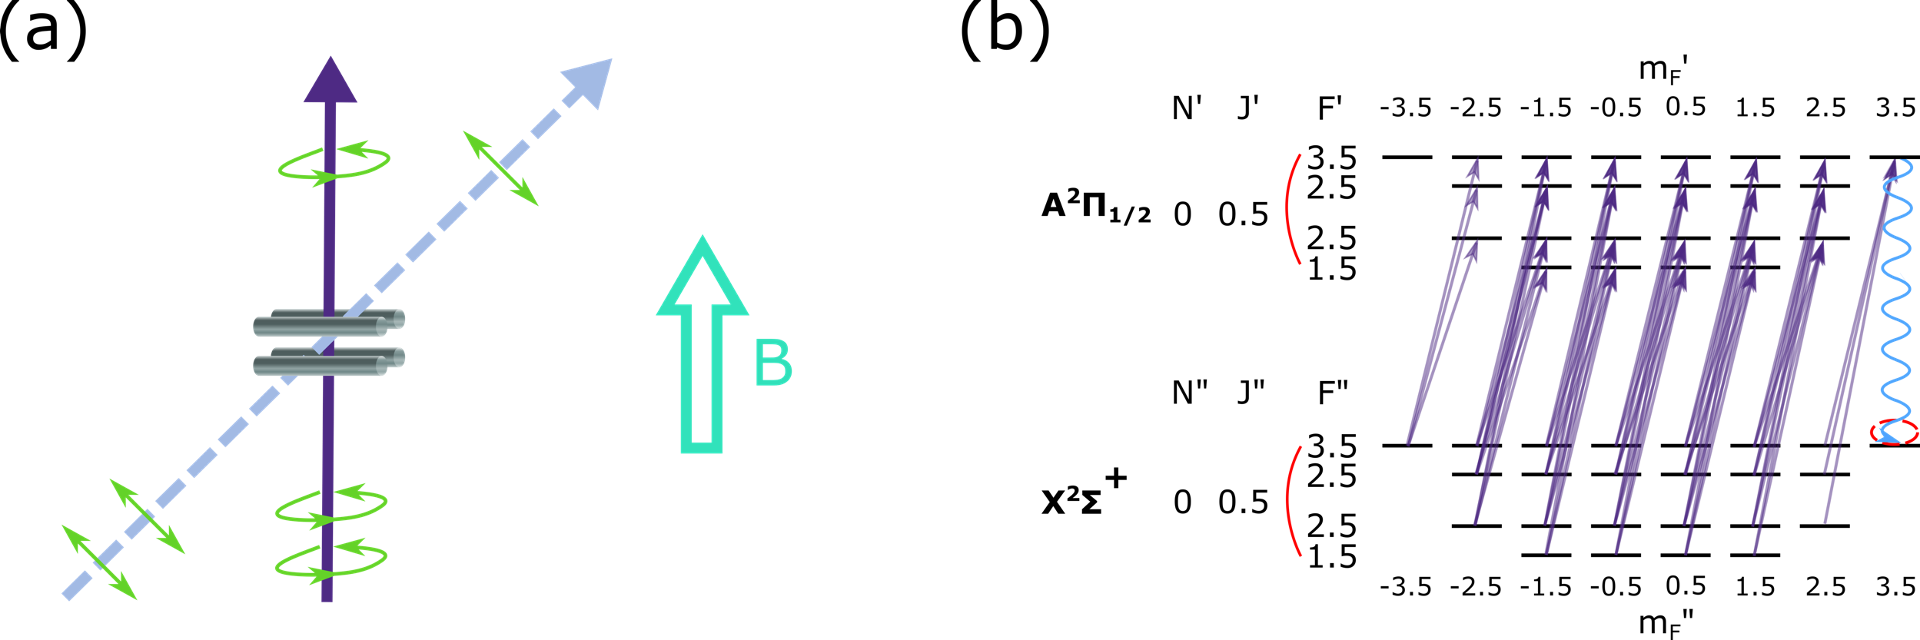
\includegraphics[width=14cm]{schematic_setup}
  \caption
  {(a) The schematic setup and (b) the hyperfine structure of the rovibrational ground state in $X^2\Sigma^+$ and $A^2\Pi_{1/2}$. In (a), rods of a linear Paul trap and two PFLs are shown. The dashed light-blue arrow indicates the linearly-polarized PFL that performs rotational cooling. The solid puple arrow indicates the $\sigma^+$-polarized PFL that drives the population into the stretched hyperfine state in the ground rovibrational manifold. In (b), the hyperfine structure and transition driven by the $\sigma^+$-polarized PFL are shown. We can see how the population in the rovibrational ground state in $X^2\Sigma^+$ is driven toward the only dark state, $\lvert X^2\Sigma^+, v=0, N=0, F''=3.5, m_{F''}=3.5\rangle$.
}\label{schematic_setup}
\end{figure*}
\section{Introduction}
%applicaitons
In recent years, molecules gradually play important roles in many applications including precision measurement\cite{kobayashi2019measurement, andreev2018improved, biesheuvel2016probing}, quantum simulation\cite{ohmori2017special}, quantum information processing\cite{grandstrand:2004, soderberg2009ultracold} and cold chemistry\cite{balakrishnan2016perspective, bohn2017cold}. In the measurement of the time-variation of $m_p/m_e$, the sensitivity to the variation of can be enhanced for the transition between two nearly degenerate vibrational levels associated with different electronic potentials of molecules\cite{demille2008enhanced, kobayashi2019measurement}. The rich internal degrees of freedom and the long-range dipole-dipole interaction between polar molecules offer possibilities of developing the quantum toolkit in both quantum simulation and quantum information processing\cite{wei2011entanglement}. Chemical interaction process can be fundamentally controlled by preparing the reactants to the certain initial external and the internal states\cite{de2011controlling}. Therefore, being able to prepare molecules to targeted initial quantum states is essential in these applications.\par
We choose to study the laser cooling the internal degrees of freedom of molecular ions in this work because in addition to the preferable nature of molecule mentioned above, the long interrogation time provided by the ion trap allows us to do a better control and study a broader set of molecules.
% Others
There have been previous efforts to achieve a single populated quantum state of neutral molecules. Some groups have performed single quantum-state preparation in the process of synthesizing molecules through photo-association of atoms followed by an stimulated Raman adiabatic transition\cite{ospelkaus2008efficient, park2015ultracold}. In their works, the constituent atoms of the molecules were trapped in a magneto-optical trap (MOT) before synthesis. The conversion efficiencies were reported to be around 75 $\%$ and 84 $\%$, respectively.\par
The controlled cooling of the population in certain hyperfine states of the molecular ion, HD$^+$ has also been demonstrated\cite{bressel2012manipulation}. Rotational cooling was accomplished by optically-pumping selected rovibrational transitions in competition with transitions induced by blackbody radiation (BBR) redistributed the population across lower vibrational states\cite{schneider2010all}. In fact, the rotational cooling timescale was limited by the BBR redistribution rate ($\sim$ 1 s). Their experimental demonstration realized a 75 $\%$ rovibrational ground-state population within tens of seconds. Manipulation of the population at the hyperfine level was then performed by coupling individual hyperfine states within the pumped rovibrational levels. A selected hyperfine state was addressed by pumping a connecting transition with a frequency-comb continuous-wave laser. The hyperfine population transfer process took a few tens of seconds.\par
%Ours
Our group has previously shown that rotational cooling of diatomic molecules can be achieved using only a pulse-shaped femtosecond laser (PFL) for species that have relatively-large rotational constants and fairly-diagonal Frank-Condon factors (FCFs)\cite{lien2011optical}. One such example is AlH$^+$, where we demonstrated the rotational ground-state population increased from a few percent to $\sim$ 95.4 $\%$ within a second.\cite{lien2014broadband} However, PFL-driven rotational cooling offers limited ability to prepare population in a single quantum state in systems that exhibit hyperfine structure in their rovibronic manifolds. For example, AlH$^+$ has one unpaired electron (electron spin $S=\frac{1}{2}$), and nuclei with nuclear spins $I_{1}=\frac{5}{2}$ and $I_{2}=\frac{1}{2}$. In the rovibronic state ($N=0$), since $J=N+S$, $F_{1}=J+I_{1}$, $F=F_{1}+I_{2}$, AlH$^{+}$ has four hyperfine states which are $F=\frac{3}{2},\, \frac{5}{2}$ states for $F_{1}=2$ and $F=\frac{5}{2},\, \frac{7}{2}$ states for $F_{1}=3$.\par
In this article, we proposed a method to further transfer the population to a single stretched hyperfine state of the rovibronic ground state in an efficient way. In Section II, we will explain the theory and our method of performing optically-driven and vibrationally-enhanced rotational-cooling. We then present our design to extend our selectivity and optically-pump the system to a single stretched hyperfine state. The simulation details will be described in Section III while Section IV presents our simulation results and discussion. We conclude in Section V.\par

%past work
%the work in this paper
%https://journals.aps.org/prl/abstract/10.1103/PhysRevLett.108.183003

\section{Theory and Methods}
\subsection{Rotational Cooling}

The time-scale of the aforementioned HD$^+$ rotational-cooling was intrinsically limited to a few tens of seconds due to the low BBR-induced transition rate. Our group has previously demonstrated broadband rotational-cooling of AlH$^+$ molecules using a linearly-polarized PFL with 100-fs pulse centered at 360 nm. The pulse is generated from a frequency-doubled femtosecond laser (Spectra-Physics Mai Tai) with 80-MHz repetition rate, so the pulse spectrum is divided into a frequency-comb with 80-MHz spacing between neighboring teeth. Its large bandwidth can pump many rotational transitions simultaneously. We use frequency-domain pulse-shaping to selectively excite cooling transitions ($\Delta N=-1$) in the rotational spectrum of the sample. As a result of the large vibrational frequency of hydrides, we focus our attention on the rotational manifolds of the ground vibrational states of the connected electronic states. As we discuss later, however, this does not mean that excited vibrational populations are not produced.%We drive the selected P- and Q- branch of electronic transition of AlH$^+$ from $\lvert X^2\Sigma^+, v''=0\rangle$ to $\lvert A^{2}\Pi, v'=0\rangle$.\par

For the purpose of discussion, we define our relevant quantum numbers to describe the states of AlH$^+$. In its ground electronic state, $X^2\Sigma^+$ state, the various angular momenta of AlH$^+$ are well-described as decoupled (Hund's case (b)), with good quantum numbers  $\left\lbrace\right.\! \Lambda, N, S, J, P \!\left.\right\rbrace$. In contrast, in its $A^2\Pi$  electronic state, AlH$^+$ is better described using the Hund's case (a) basis of $\left\lbrace\right.\! \Lambda, S, \Sigma, J, \Omega, \mathit{P} \!\left.\right\rbrace$. This means that electronic transitions do not always yield consistent and clear selection rules for $N$. For convenience, we will generally describe rotational transitions (and thus, cooling transitions) as changes to $N$, which has different meaning for the $X^2\Sigma^+$ and the $A^2\Pi$ states. In $X^2\Sigma^+$, $N$ represent the rotational angular momentum of the molecule except spin electronic spin. While in $A^2\Pi$, $N$ just serves as a notation to mark different J values.  Thus, our mention of P($N_i$)-, Q($N_i$)-, and R($N_i$)-branch transitions refer to changes in $N$ of -1, 0, and +1, respectively, with respect to the initial state, $N_i$. It should be noted that the rotational states of both the X and A states of AlH$^+$ are organized into parity doublets. In the X state, the doubling is a result of electron spin-molecular rotation interaction while the doubling in the $A^2\Pi$ state is produced by the interaction between the rotation of the nuclei $L$, also known as $\Lambda$-type  doubling. For both electronic states, $v$ is the vibrational quantum number. We invoke the convention that $v'$ ($v''$) denotes the vibrational quantum number of the upper (lower) state.

The rotational cooling process has two parts. The first part is a fast cycle in which linearly-polarized 360-nm pulses of the PFL drive the electronic transition connecting $\lvert X^2\Sigma^+, v''=0\rangle$ and $\lvert A^{2}\Pi_{1/2}, v'=0\rangle$. Followed by the excitation, laser-induced stimulated emission and spontaneous emission with the relaxation time around 60 ns from the A state occurs.  Initially, there is significant rotational population in the lowest 10 rotational states. Nearly all of it can be driven into the two lowest rotational states, $\lvert v''=0, N''=0,1\rangle$, within only a few microseconds. However, parity is flipped for a dipole-transitions such as $\lvert X^2\Sigma^+\rangle \leftrightarrow \lvert A^2\Pi\rangle$. As a result, the population in $\lvert X^2\Sigma^+, v''=0, N''=1, -\rangle$ cannot be transferred to the rovibronic ground state, $\lvert X^2\Sigma^+, v''=0, N''=0, +\rangle$ via this fast electronic cooling cycle in which the parity is conserved after flipping twice. The population in $\lvert X^2\Sigma^+, v''=0, N''=1, -\rangle$ can still relax to the rovibronic ground state, but must do so in an odd number of transitions. In the simplest case, the negative-parity rotational populations are transferred to the positive-parity rovibronic ground state in three transitions. After excitation by the PFL, each population can pass through an intermediate state of negative parity, $\lvert X^2\Sigma^+, v''=1, N''=1, -\rangle$ (as shown in Figure \ref{level_diagram_parity}). This "parity-flipping process", which constitutes the second part of the cooling process, is relatively slow because the vibrational relaxation time for the $\lvert X^2\Sigma^+, v=1\rangle \leftrightarrow \lvert X^2\Sigma^+, v=0\rangle$ transition is about 140 ms.

In our laboratory, AlH$^+$ ions are trapped in a linear Paul trap and initially sympathetically-cooled to sub-Kelvin translational temperatures using co-trapped Doppler-cooled Ba$^+$. To remove the dark states of barium ion during the Doppler-cooling process, a 2-G magnetic field is applied. After translational cooling, the linearly-polarized PFL (laser polarization is perpendicular to the laboratory-applied magnetic field) is turned on to perform rotational cooling of the molecules into their rovibronic ground state.

We now describe our method to enhance the rotational cooling process. Previously, we recognized that cooling of the negative-parity populations is rate-limited by the vibrational decay timescale. We propose to address this bottleneck through the addition of a 6.6-{\micro}m continuous-wave laser which couples the $\lvert X^2\Sigma^+, v''=1, N''=1, -\rangle \leftrightarrow \lvert X^2\Sigma^+, v''=0, N''=2, +\rangle$ transition. We assert, based on computer simulations, that with this laser, the rotational-cooling timescale can be shortened by about three orders of magnitude (see Figure \ref{RC_RCV10} and Table \ref{RC_RC_V10table}.


\subsection{Hyperfine Cooling}
Moreover, as we are interested in pumping our system to single (hyperfine) quantum state, we also add a circularly-polarized 360-nm beam. By taking advantage of the selection rules for transitions driven by $\sigma^+$-polarized light, we can optical pump the system to a \textit{stretched} hyperfine state in which the total angular momentum ($F$) has the largest projection ($m_F$) along the quantization axis). The schematic plot of our setup is shown in Figure \ref{schematic_setup}. When we apply the $\sigma^+$-polarized laser, the selection rule are as follows:

\begin{align*}
\Delta F=0, \pm 1 \\
\Delta m_F=1
\end{align*}


As can be seen in Figure \ref{schematic_setup}, if we can park the $\sigma^+$-polarized laser to drive the hyperfine manifold within the Q$_{11}$(0)-branch transition\footnote[1]{This notation describes the branch in terms of both $N$ and $J$: $^{\Delta N}\Delta J_{ul}$. If $\Delta N = \Delta J$, then the notation uses one letter to mark the type of branch.  $u$ and $l$ denote the spin orientation of the upper state and the lower state in a transition. In our case, the upper state could be the $A^2\Pi_{1/2}$ or the $A^2\Pi_{3/2}$ state, which are denoted by $u=1$  and $u=2$ respectively. The lower state is the $X^2 \Sigma^{+}$ state with $S=1/2$. We choose the convention of $l=1$ ($l=2$) to represent $J=N+1/2$ ($J=N-1/2$).}, $\lvert X^2\Sigma^+, v''=0, N''=0\rangle \leftrightarrow \lvert A^2\Pi_{1/2}, v'=0, N'=0\rangle$, most of the population in the rovibronic ground state of $X^2 \Sigma^{+}$ will be further cooled to a single stretched hyperfine state, notably the stretched state of maximal F. This stretched hyperfine state is a dark state; it cannot absorb any more $\sigma^+$-polarized photons because there is no higher $m_F$-state available in the $\lvert A^2\Pi_{1/2}, v=0, N=0\rangle$. The population will remain in this state as long as it is not exposed to linearly- or $\sigma^-$-polarized light. Our goal of single quantum-state preparation is achieved.

\section{Simulation Details}

\begin{center}
%\begin{table*}
\begin{table*}
\begin{minipage}[b]{0.45\linewidth}
%\centering
\let\TPToverlap=\TPTrlap
\caption{Molecular constants for the $X^2\Sigma^+$ state of AlH$^{+}$\tnote{a}}
\begin{threeparttable}
\renewcommand{\arraystretch}{1.25}
\setlength{\tabcolsep}{1em}
\begin{tabular}{lcc}
%\multicolumn{3}{|c|}{WTmetaD parameters} \\
 \hline\colrule
Constant\cite{szajna2011high} &$X^2\Sigma^+$,  $ v=0$   &$X^2\Sigma^+$,  $ v=1$    \\
 \hline\colrule
$B_{v}$                                    &$6.563231$ &$6.184845$   \\   \hline
$D_{v}\times 10^{4}$              &$4.5720$     &$5.0983$      \\ \hline
$H_{v}\times 10^{8}$              &$-0.238$     &$-6.586$       \\ \hline
$L_{v}\times 10^{11}$              &$-1.712$      &                  \\ \hline
$M_{v}\times 10^{14}$            &$1.140$        &                  \\ \hline
$N_{v}\times 10^{18}$             &$-7.07$        &                  \\ \hline
$\gamma_{v}\times 10^{2}$    &$5.665$       &$5.035$        \\ \hline
$\gamma_{Dv}\times 10^{5}$  &$-1.896$     &$-2.09$        \\ \hline
Origin                                         &$0$              &$1523$        \\ 
\botrule
\end{tabular}
\begin{tablenotes}
\item[a] in $cm^{-1}$
\end{tablenotes}
\end{threeparttable}
\label{Xparameters}

\end{minipage}
\hspace{0.2cm}
\begin{minipage}[b]{0.45\linewidth}
\centering
%\end{table*}
%\end{center}

%\begin{center}
%\begin{table*}
\let\TPToverlap=\TPTrlap
\caption{Molecular constants for the $A^2\Pi$ state of AlH$^{+}$ \tnote{b}}
\renewcommand{\arraystretch}{1.25}
\begin{threeparttable}
\setlength{\tabcolsep}{1em}
\begin{tabular}{lc}
 \hline\colrule
Constant                                 &$A^2\Pi$,  $ v=0$   \\
 \hline\colrule
$B_{v}$                                   &$6.727$ \cite{almy1934band}     \\   \hline
$A_{v}$                                   &$108$ \cite{almy1934band}        \\ \hline
$p_{v}\times 10^{2}$             &$1.643$ \cite{szajna2011high}    \\ \hline
$q_{v}\times 10^{3}$             &$1.499$ \cite{szajna2011high}    \\ \hline
$D_{v}\times 10^{4}$             &$-4.14$ \cite{almy1934band}     \\ \hline
Origin                                      &$27713$ \cite{szajna2011high}   \\ 
\botrule
\end{tabular}
\begin{tablenotes}
\item[b] in $cm^{-1}$
\end{tablenotes}
\end{threeparttable}
\label{Aparameters}
%\end{table*}
%\end{center}
\end{minipage}
\end{table*}
\end{center}

\begin{center}
\begin{table*}
\let\TPToverlap=\TPTrlap
\caption{Permanent and transition dipole moments ($\langle$ State A $\lvert\,\mu\,\rvert$ State B$\rangle$) \tnote{c}}
\renewcommand{\arraystretch}{1.5}
\begin{threeparttable}
\setlength{\tabcolsep}{3pt}
\begin{tabular}{c|ccc}
%\multicolumn{3}{|c|}{WTmetaD parameters} \\
 \hline\colrule
\diagbox{State A}{State B}           &$X^2\Sigma^+, v=0$     &$X^2\Sigma^+, v=1$    &$A^2\Pi, v=0$  \\ 
 \hline\colrule
$X^2\Sigma^+, v=0$                     &$-0.389$                        &                                       & \\   \hline
$X^2\Sigma^+, v=1$                      &$0.087$                          &$-0.2861$                     &\\ \hline
$A^2\Pi, v=0$                                 &$1.566$                          &$-0.2806$                    &$-0.928$\\ 
\botrule
\end{tabular}
\begin{tablenotes}
\item[c] in Debye
\end{tablenotes}
\end{threeparttable}
\label{dipolemoment}
\end{table*}
\end{center}


\begin{center}
\begin{table*}[htbp!]
\let\TPToverlap=\TPTrlap
\caption{Hyperfine constants of AlH$^{+}$ in terms of Frosch-Foley coefficients and parameters of nuclear quadrupole interaction\tnote{d}}
\renewcommand{\arraystretch}{1.5}
\begin{threeparttable}
\setlength{\tabcolsep}{6pt}
\begin{tabular}{*{5}{c}}
%\multicolumn{3}{|c|}{WTmetaD parameters} \\
\hline\colrule
\multirow{2}{*}{Constant} &\multicolumn{2}{c}{$X^2\Sigma^+$} &\multicolumn{2}{c}{$A^2\Pi$} \\
\cline {2-5}
&Al &H  &Al &H\\
 \hline\colrule
a               &\num{1.680E-3}           &\num{8.64E-5}            &\num{8.511E-3}              &\num{5.53E-4}         \\
b               &\num{3.951E-2}           &\num{2.01E-2}             &\num{1.382E-2}             &\num{-9.35E-3}         \\
c               &\num{5.039E-3}          &\num{2.59E-4}             &\num{-5.654E-3}            &\num{2.79E-4}         \\
d               &\num{0}                        &\num{0}                         &\num{1.040E-2}             &\num{4.60E-4}          \\
$eQq0$    &\num{-1.341211E-3}    &\num{2.12636E-6}        &\num{6.20358E-4}       &\num{2.34231E-6}      \\
$eQq2$    &\num{0}                        &\num{0}                          &\num{-2.896517E-3}    &\num{-5.63315E-7}     \\               
\botrule
\end{tabular}
\begin{tablenotes}
\item[d] in cm$^{-1}$
\end{tablenotes}
\end{threeparttable}
\label{hyperfineconstant}
\end{table*}
\end{center}

Our population dynamics are calculated through the following rate equation:
\begin{align}
\begin{aligned}
\frac{\partial\rho_i}{\partial t}=-\sum_{j\neq i}B_{i,j}(I_{BBR}+I_{laser})\rho_i - \sum_{j<i}A_{i,j}\rho_i \\
+\sum_{j\neq i}B_{j,i}(I_{BBR}+I_{laser})\rho_i + \sum_{j>i}A_{j,i}\rho_i 
\end{aligned}
\end{align}
where $\rho_i$ is the population fraction in state $i$. The initial population is assumed to be thermal with a temperature of 300 K. $I_{BBR}$ and $I_{laser}$ are the energy densities of the blackbody radiation and laser. A and B are the spontaneous emission and stimulated emission Einstein coefficients, respectively.
\begin{align}
\begin{aligned}
A_{ul} = \frac{2\pi \widetilde{\nu}^2 q_e^2}{\epsilon_0 m_e c} \frac{g_l}{g_u} f_{lu}\\
B_{ul} = \frac{q_e^2}{4 \epsilon_0 m_e h c \widetilde{\nu}} \frac{g_l}{g_u} f_{lu} \\
B_{lu} = \frac{q_e^2}{4 \epsilon_0 m_e h c \widetilde{\nu}} f_{lu}\\
\end{aligned}
\end{align}
In order to determine the Einstein coefficients using Equation (2), we utilize Western's PGOPHER\cite{western2017pgopher} software to compute transition energies and oscillator strengths for a single AlH$^+$ molecule in a 10-G laboratory-frame magnetic field. 

We require a number of empirical parameters that describe the states of the AlH$^+$ molecule. Table \ref{Xparameters} and \ref{Aparameters} present the empirical values used throughout this work to describe the $X^2 \Sigma^{+}$  and $A^2\Pi_{1/2}$ states.

Additionally, we use Le Roy's LEVEL\cite{le2017level} to calculate the permanent and transition electric-dipole moments from the potential-energy functions and transition-dipole-moment functions calculated in the supplementary data of a prior work\cite{nguyen2011challenges}. The calculated result is shown in Table \ref{dipolemoment}.

Dalton\cite{daltonpaper, daltonwebpage} quantum computational software was used to compute hyperfine and nuclear-quadrupole coupling constants of the $X^2\Sigma+$ and $A^2\Pi$ states, which are listed in Table \ref{hyperfineconstant}. We choose the pcJ-1 basis set because pcJ family was developed for RMN/EPR spin-spin coupling constants and have tight functions that are well suited for describing the electron density near the nucleus. Density Functional Theory (DFT) using the B3LYP density functional is applied with an pcJ-1 basis set for all computations.

At room temperature, 99 $\%$ of the AlH$^+$ population is in the lowest vibrational state, $v=0$ within the $X^2 \Sigma$ manifold. Within this vibronic ground state, there is significant population thermally-distributed among the first ten J-levels, $J=0.5$-$9.5$, and less than $4\, \%$ in $J>9.5$. Therefore, we include only these lowest ten J-states in our rate-equation simulation for both the X and A states. We also include the $X^2\Sigma+ (v''=1)$ manifold so that we can simulate the parity-flipping process via the intermediate state, $\lvert X^2\Sigma^+, v''=1, N''=1, -\rangle$.

Our femtosecond laser has a frequency-domain representation in the simulation. The spectrum is described by 80-MHz-spaced comb teeth within a Gaussian envelope that is centered at 360 nm and has a $\sim$7-nm FWHM bandwidth. We model our pulse-shaping apparatus as a cut-off to the laser spectrum. The cut-off frequency is chosen so as to pass the range of frequencies that selectively drives a set of rotational-cooling transitions. For example, we choose to drive the $P_{11}$, $^OP_{12}$ and the $^PQ_{12}$ branches using the linearly-polarized PFL and then include the $Q_{11}(0)$ branch for the $\sigma^+$-polarized PFL. We assume a 200-mW power split equally between the linear- and the $\sigma^+$-polarized beams with a focused 400-{\micro}m-diameter spot at the position of AlH$^+$ molecules.

The typical optical transition linewidth for AlH$^+$ is $\sim$20 MHz, which is smaller than the 80-MHz comb-teeth spacing of the femtosecond laser spectrum. As a result, it is possible the PFL comb lines are detuned with more than the transition linewidth from some the transitions we desire to drive. We solve this issue in the simulation by introducing a Doppler-broadened linewidth contribution that assumes the translational temperature of the AlH$^+$ ion cloud is $\sim 1\, K$. Doing so ensures that there is at least one comb line within the linewidth of every desired cooling transition. One can accomplish this form of broadening in the experiment by raising the translational temperature of the AlH$^+$ ions in a couple ways. One can excite the secular motion of the AlH$^+$ with an AC field or introduce more micro motions by shifting the entire ion cloud away from the geometric center of the Paul trap using a DC field. After internal cooling is finished, one can then turn off the source of translational heating to allow sympathetic-cooling by the laser-cooled Ba$^+$.


\begin{figure*}[htbp!]
  \centering
  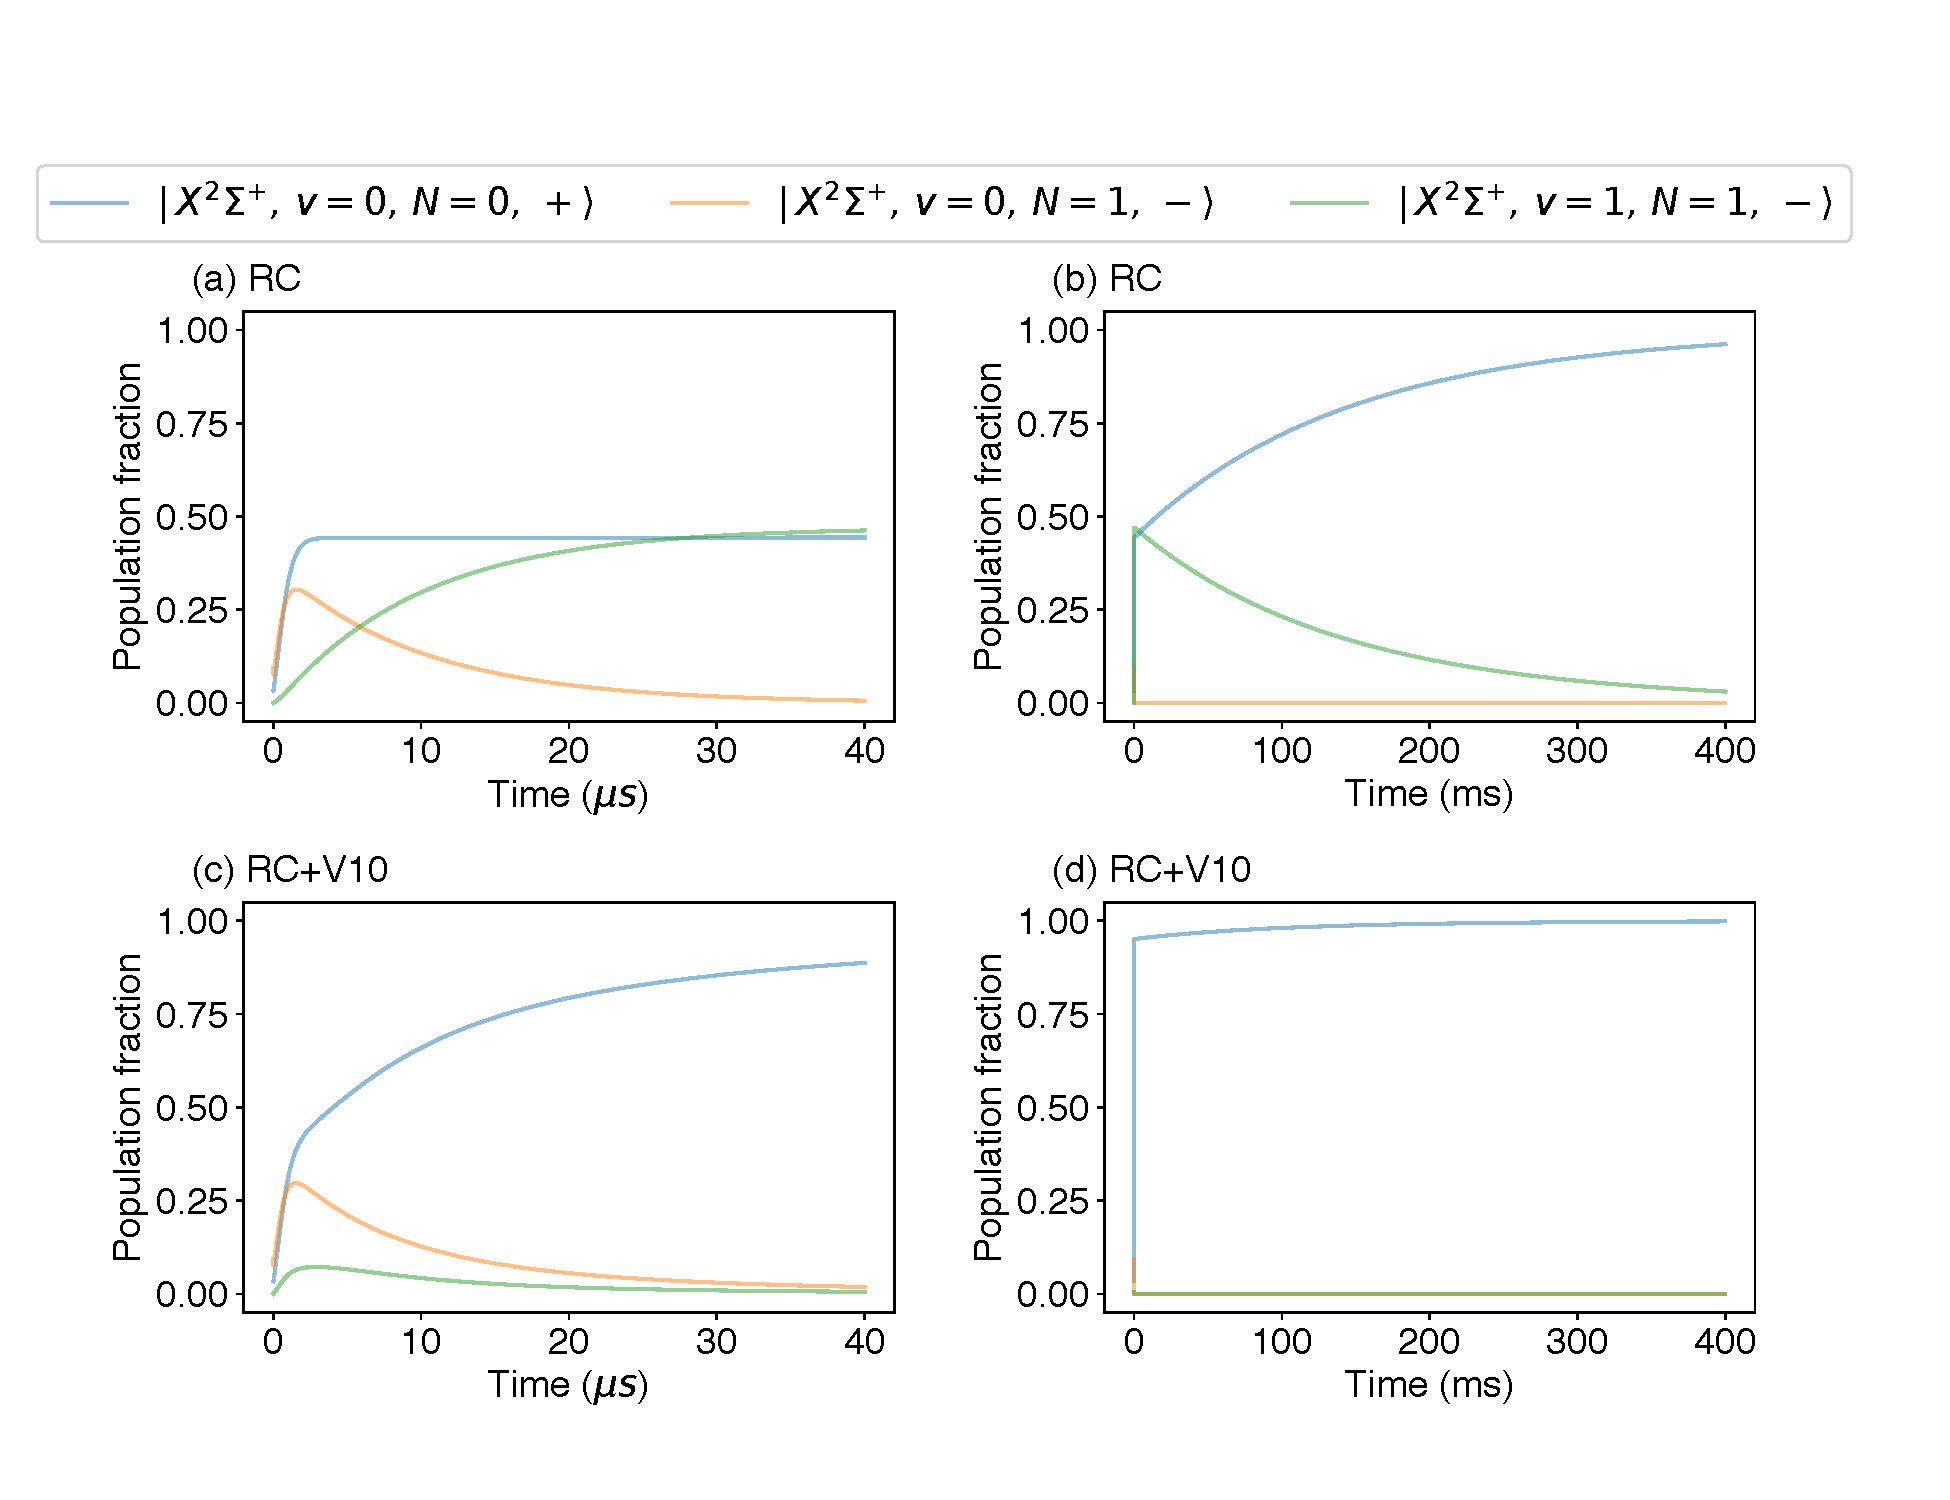
\includegraphics[width=12cm]{RC_RCV10}
  \caption
  {Simulated population dynamics for rotational-cooling: The top two plots are for the cases in which only the linearly-polarized rotational-cooling PFL (RC) was applied for (a) 40 {\micro}s and (b) 400 ms, respectively. The bottom two plots describe rotational-cooling via the PFL but now with the additional laser (V10) to drive the $\lvert X^2\Sigma^+, v''=1, N''=1, -\rangle \leftrightarrow \lvert X^2\Sigma^+, v''=0, N''=2, +\rangle$ transition, for (c) 40 {\micro}s and (d) 400 ms, respectively.
  }\label{RC_RCV10}
\end{figure*}

\begin{figure*}[htbp!]
  \centering
  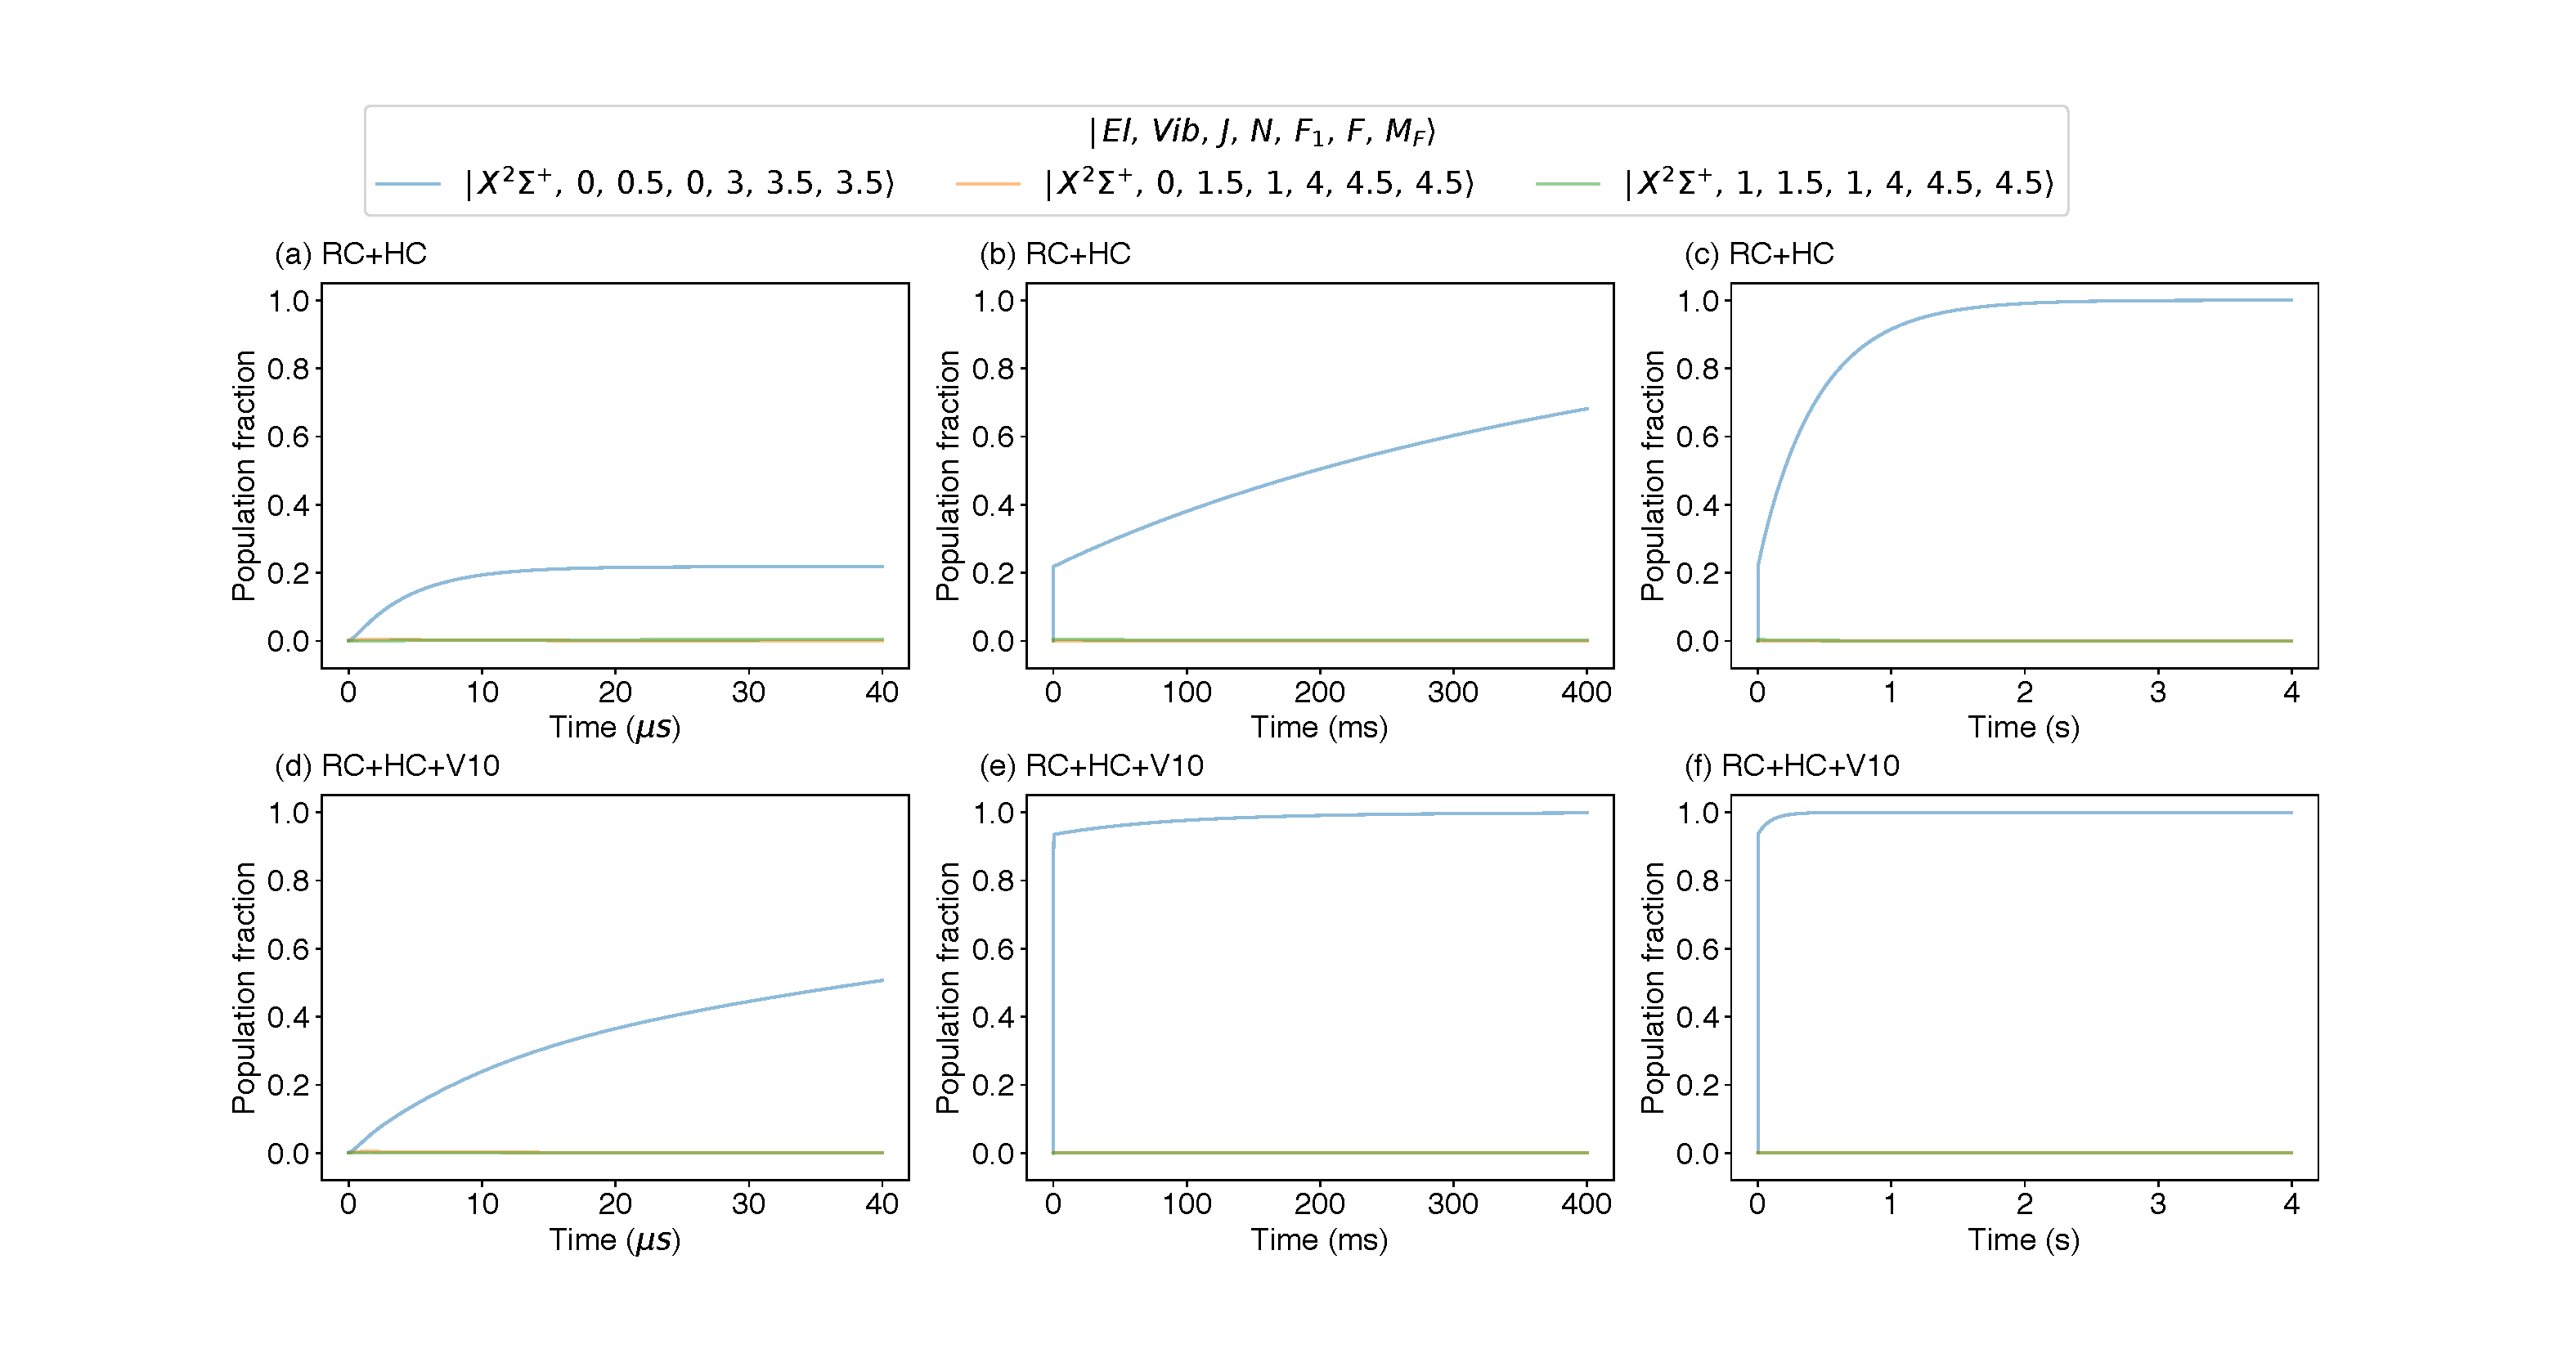
\includegraphics[width=18cm]{RCHC_RCHCV10}
  \caption
  {Simulated population dynamics for preparation of a single hyperfine state: The top three plots are for the cases in which the linearly-polarized rotational-cooling PFL (RC) and the $\sigma^+$-polarized hyperfine-cooling PFL are applied for (a) 40 {\micro}s, (b) 400 ms, and (c) 4 s, respectively. The bottom two plots describe rotational- and hyperfine-cooling via the linearly- and circularly-polarized PFLs but now with the additional laser (V10) to drive the $\lvert X^2\Sigma^+, v''=1, N''=1, -\rangle \leftrightarrow \lvert X^2\Sigma^+, v''=0, N''=2, +\rangle$ transition, for (d) 40 {\micro}s, (e) 400 ms, and (f) 4 s  respectively.
}\label{RCHC_RCHCV10}
\end{figure*}


\begin{table*}[!htbp]
\begin{minipage}[b]{0.45\linewidth}
\renewcommand{\arraystretch}{1.25}
\caption{The time for the rovibronic ground-state population to reach $63.2$ $\%$ and $95.4$ $\%$.}
\setlength{\tabcolsep}{6pt}
\begin{tabular}{c|cc}
%\hline
%\multicolumn{3}{|c|}{WTmetaD parameters} \\
\hline\colrule
Laser fields & $63.2$ $\%$ &  $95.4$ $\%$   \\ 
\hline\colrule
RC & $60.0$ ms & $371.4$ ms \\ \hline
RC, V10 & $9.5$ {\micro}s & $680.0$ {\micro}s \\ 
\botrule
\end{tabular}
\label{RC_RC_V10table}

\end{minipage}
\hspace{0.2cm}
\begin{minipage}[b]{0.45\linewidth}

\renewcommand{\arraystretch}{1.25}
\caption{The time for the hyperfine stretched-state population to reach $63.2$ $\%$ and $95.4$ $\%$.}
\setlength{\tabcolsep}{6pt}
\begin{tabular}{c|cc}
%\hline
%\multicolumn{3}{|c|}{WTmetaD parameters} \\
\hline\colrule
Laser fields & $63.2$ $\%$ &  $95.4$ $\%$   \\ 
\hline\colrule
RC, HC &$334.6$ ms & $1280$ ms \\ \hline
RC, HC, V10 & $80.0$ {\micro}s & $2.2$ ms \\
\botrule
\end{tabular}
\label{RCHC_RCHCV10table}
\end{minipage}
\end{table*}



We simulate the vibrationally-enhanced parity-flipping processes as well. For such cases, we represent the laser (V10) that drives the $\lvert X^2\Sigma^+, v''=1, N''=1, -\rangle \leftrightarrow \lvert X^2\Sigma^+, v''=0, N''=2, +\rangle$ transition to match the specifications of a commercial Fabry-Perot quantum-cascade laser (ThorLabs model number). The laser has a $\sim$15-cm$^{-1}$ bandwidth centered at $\sim$6.6 {\micro}m, which overlaps well with the transition energy of the $v''=0 \leftrightarrow v'=1$ band in the electronic ground state of AlH$^+$.

\section{Result and discussion}
Figure \ref{RC_RCV10} and Table \ref{RC_RC_V10table} present rotational-cooling rates for two schemes. In the first scheme, we apply the linearly-polarized rotational-cooling laser (RC). In the second scheme, we apply the rotational-cooling laser (RC) as well as a laser (V10) that drives the $\lvert X^2\Sigma^+, v''=1, N''=1, -\rangle \leftrightarrow \lvert X^2\Sigma^+, v''=0, N''=2, +\rangle$ transition. The addition of the V10 laser clearly reduces the time it takes for the population in the rovibronic ground state, p$_0$, to grow to 63.2 $\%$, as it is shortened from 49.5 ms to 9.4 {\micro}s. The trend continues as p$_0$ reaches 95.4 $\%$, which takes only 49.5 ms, a factor of six smaller than the 307.4 ms required in the absence of the rovibrational couple.

Figure \ref{RCHC_RCHCV10} and Table \ref{RCHC_RCHCV10table} present our simulation results for two hyperfine-cooling schemes. In the first scheme, we apply the rotational-cooling laser (RC) and the $\sigma^+$-hyperfine-cooling laser (HC). In the second scheme, we apply the hyperfine-cooling laser (HC) as well as the rovibrational coupling laser (V10). In the absence of the V10 laser, the population in the stretched hyperfine state increases to $\sim 20 \%$ during the first tens of microsecond. There is also a longer dynamical timescale. We see that after a second, the population has reached more than 90 $\%$, exceeding the theoretical-maximum population of $65 \%$ reported in the previous work using HD$^+$\cite{bressel2012manipulation}. When the V10 laser is also applied, the time it takes for the stretched hyperfine-state population in the rovibronic ground state, p$_{0s}$, to reach 63.2 $\%$ is shortened from 276.2 ms to 80.0 {\micro}s. If we leave the lasers on, p$_{0s}$ can reach 95.4 $\%$ in 2.0 ms with the rovibrational couple, a 500-fold reduction from the 1058-ms rise-time in its absence.

\section{Conclusion}
We have described a method to achieve faster and more selective internal-state cooling in the molecular ion, AlH$^+$. We based on design on the simple premise that in order to speed up the cooling process, we have to accelerate the rate-limiting step. In the AlH$^+$ system, the rate-limiting step is the parity-flipping process. We expect to accomplish this task by adding a new laser field that drives population out of the intermediate state. We further describe an extension to our previous rotational-cooling work that should enable one to drive population to a single hyperfine state. We exploit the selection rules of a circularly-polarized laser field in a simulation and find a noteworthy result: we should be able to prepare AlH$^+$ molecules in a single quantum state in about a second. Faster dynamics are likely to be achievable with more intense lasers.

\bibliographystyle{ieeetr}
\bibliography{../AlH+_references.bib}

\end{document}